%beamer

% Dieser Foliensatz wurde noch nicht überarbeitet, da es nur 14 Tutorien gab.

% Define a global usable date. Must come before StyleTut
%\newcommand{\mydate}{05.02.2013}

% Comment/uncomment this line to toggle handout mode
%\newcommand{\handout}{}

%% Beamer-Klasse im korrekten Modus
\ifdefined \handout
\documentclass[handout]{beamer} % Handout mode
\else
\documentclass{beamer}
\fi

%% UTF-8-Encoding
\usepackage[utf8]{inputenc}

\input{../framework/gbi-macros}
\usepackage[blue]{../framework/thwregex}
\usepackage{environ}
\usepackage{bm}
\usepackage{calc}
\usepackage{varwidth}
\usepackage{wasysym}
\usepackage{mathtools}


% Das ist der KIT-Stil
%\usepackage{../TutTexbib/beamerthemekit}
\usepackage[deutsch,titlepage0]{../framework/KIT/beamerthemeKITmod}
\TitleImage[width=\titleimagewd]{../figures/titlepage.jpg}
%\usetheme[deutsch,titlepage0]{KIT}

% Include PDFs
\usepackage{pdfpages}

% Libertine font (Original GBI font)
\usepackage{libertine}
%\renewcommand*\familydefault{\sfdefault}  %% Only if the base font of the document is to be sans serif

% Nicer math symbols
\usepackage{eulervm}
%\usepackage{mathpazo}
\renewcommand\ttdefault{cmtt} % Computer Modern typewriter font, see lecture slides.

\usepackage{csquotes}

%%%%%%

%% Schönere Schriften
\usepackage[TS1,T1]{fontenc}

%% Bibliothek für Graphiken
\usepackage{graphicx}

%% der wird sowieso in jeder Datei gesetzt
\graphicspath{{../figures/}}

%% Anzeigetiefe für Inhaltsverzeichnis: 1 Stufe
\setcounter{tocdepth}{1}

%% Hyperlinks
\usepackage{hyperref}
% I don't know why, but this works and only includes sections and NOT subsections in the pdf-bookmarks.
\hypersetup{bookmarksdepth=subsection} 

%\usepackage{lmodern}
\usepackage{colortbl}
\usepackage[absolute,overlay]{textpos}
\usepackage{listings}
\usepackage{forloop}
%\usepackage{algorithmic} % PseudoCode package 

\usepackage{tikz}
\usetikzlibrary{matrix}
\usetikzlibrary{arrows.meta}
\usetikzlibrary{automata}
\usetikzlibrary{tikzmark}
\usetikzlibrary{positioning}

% Why has no-one come up with this yet? I mean, seriously. -.-
\tikzstyle{loop below right} = [loop, out=-60,in=-30, looseness=7]
\tikzstyle{loop below left} = [loop, out=-150,in=-120, looseness=7]
\tikzstyle{loop above right} = [loop, out=60,in=30, looseness=7]
\tikzstyle{loop above left} = [loop, out=150,in=120, looseness=7]
\tikzstyle{loop right below} = [loop below right]
\tikzstyle{loop left below} = [loop below left]
\tikzstyle{loop right above} = [loop above right]
\tikzstyle{loop left above} = [loop above left]

% Needed for gbi-macros
\usepackage{xspace}

%%%%%%

%% Verbatim
\usepackage{moreverb}

%%%%%%%%%%%%%%%%%%%%%%%%%%%%%%%%%%%% Copy end

%% Tabellen
\usepackage{array}
\usepackage{multicol}
\usepackage{hhline}

%% Bibliotheken für viele mathematische Symbole
\usepackage{amsmath, amsfonts, amssymb}

%% Deutsche Silbentrennung und Beschriftungen
\usepackage[ngerman]{babel}

\usepackage{kbordermatrix}

% kbordermatrix settings
\renewcommand{\kbldelim}{(} % Left delimiter
\renewcommand{\kbrdelim}{)} % Right delimiter

\input{../config.tex}



% define custom \handout command flag if handout mode is toggled  #DirtyAsHellButWell...
\only<beamer:0>{\def\handout{}} %beamer:0 == handout mode

\newcommand{\R}{\mathbb{R}}
\newcommand{\N}{\mathbb{N}}
\newcommand{\Z}{\mathbb{Z}}
\newcommand{\Q}{\mathbb{Q}}
\newcommand{\BB}{\mathbb{B}}
\newcommand{\C}{\mathbb{C}}
\newcommand{\K}{\mathbb{K}}
\newcommand{\G}{\mathbb{G}}
\newcommand{\nullel}{\mathcal{O}}
\newcommand{\einsel}{\mathds{1}}
\newcommand{\Pot}{\mathcal{P}}
\renewcommand{\O}{\text{O}}

\def\word#1{\hbox{\textcolor{blue}{\texttt{#1}}}}
\let\literal\word
\def\mword#1{\hbox{\textcolor{blue}{$\mathtt{#1}$}}}  % math word
\def\sp{\scalebox{1}[.5]{\textvisiblespace}}
\def\wordsp{\word{\sp}}

%\newcommand{\literal}[1]{\textcolor{blue}{\texttt{#1}}}
\newcommand{\realTilde}{\textasciitilde \ }
\newcommand{\setsize}[1]{\ensuremath{\left\lvert #1 \right\rvert}}
\newcommand{\size}[1]{\setsize{#1}}  % Shame on you, TeXStudio...
\newcommand{\set}[1]{\left\{#1\right\}}
\newcommand{\tuple}[1]{\left(#1\right)}
\newcommand{\normalvar}[1]{\text{$#1$}}

% Modified by DJ
\let\oldemptyset\emptyset
\let\emptyset\varnothing % proper emptyset

\newcommand{\boder}{\ensuremath{\mathbin{\textcolor{blue}{\vee}}}\xspace}
\newcommand{\bund}{\ensuremath{\mathbin{\textcolor{blue}{\wedge}}}\xspace}
\newcommand{\bimp}{\ensuremath{\mathrel{\textcolor{blue}{\to}}}\xspace}
\newcommand{\bgdw}{\ensuremath{\mathrel{\textcolor{blue}{\leftrightarrow}}}\xspace}
\newcommand{\bnot}{\ensuremath{\textcolor{blue}{\neg}}\xspace}
\newcommand{\bone}{\ensuremath{\textcolor{blue}{1}}\text{}}
\newcommand{\bzero}{\ensuremath{\textcolor{blue}{0}}\text{}}
\newcommand{\bleftBr}{\ensuremath{\textcolor{blue}{\texttt{(}}}\text{}}
\newcommand{\brightBr}{\ensuremath{\textcolor{blue}{\texttt{)}}}\text{}}

% Fix of \b... commands:

\renewcommand{\boder}{\alor}
\renewcommand{\bund}{\aland}
\renewcommand{\bimp}{\alimpl}
\renewcommand{\bgdw}{\aleqv}
\renewcommand{\bnot}{\alnot}
\renewcommand{\bleftBr}{\alka}
\renewcommand{\brightBr}{\alkz}
\newcommand{\alA}{\word A}
\newcommand{\alB}{\word B}
\newcommand{\alC}{\word C}

\newcommand{\plB}{\plfoo{B}}
\newcommand{\plE}{\plfoo{E}}

\newcommand{\summe}[2]{\sum\limits_{#1}^{#2}}
\newcommand{\limes}[1]{\lim\limits_{#1}}

%\newcommand{\numpp}{\advance \value{weeknum} by -2 \theweeknum \advance \value{weeknum} by 2}
%\newcommand{\nump}{\advance \value{weeknum} by -1 \theweeknum \advance \value{weeknum} by 1}

\newcommand{\mycomment}[1]{}
\newcommand{\Comment}[1]{}

%% DISCLAIMER START 
% It is INSANELY IMPORTANT NOT TO DO THIS OUTSIDE BEAMER CLASS! IN ARTCILE DOCUMENTS, THIS IS VERY LIKELY TO BUG AROUND!
\makeatletter%
\@ifclassloaded{beamer}%
{
	% TODO 
	% no time... later.   (= never -.-)
	% redefine section to ignore multiple \section calls with the same title
}%
{
	\errmessage{ERROR: section command redefinition outside of beamer class document! Please contact the author of this code or read the F-ing disclaimer.}
}%
\makeatother%
%% DISCLAIMER END

\newcounter{abc}
\newenvironment{alist}{
  \begin{list}{(\alph{abc})}{
      \usecounter{abc}\setlength{\leftmargin}{8mm}\setlength{\labelsep}{2mm}
    }
}{\end{list}}


\newcommand{\stdarraystretch}{1.20}
\renewcommand{\arraystretch}{\stdarraystretch}  % for proper row spacing in tables

\newcommand{\morescalingdelimiters}{   % for proper \left( \right) typography
	\delimitershortfall=-1pt  
	\delimiterfactor=1
}

\newcommand{\centered}[1]{\vspace{-\baselineskip}\begin{center}#1\end{center}\vspace{-\baselineskip}}

% for \implitem and \item[bla] stuff to look right:
\setbeamercolor*{itemize item}{fg=black}
\setbeamercolor*{itemize subitem}{fg=black}
\setbeamercolor*{itemize subsubitem}{fg=black}

\setbeamercolor*{description item}{fg=black}
\setbeamercolor*{description subitem}{fg=black}
\setbeamercolor*{description subsubitem}{fg=black}

\renewcommand{\qedsymbol}{\textcolor{black}{\openbox}}

\renewcommand{\mod}{\mathop{\textbf{mod}}}
\renewcommand{\div}{\mathop{\textbf{div}}}

\newcommand{\ceil}[1]{\left\lceil#1\right\rceil}
\newcommand{\floor}[1]{\left\lfloor#1\right\rfloor}
\newcommand{\abs}[1]{\left\lvert #1 \right\rvert}
\newcommand{\Matrix}[1]{\begin{pmatrix} #1 \end{pmatrix}}
\newcommand{\braced}[1]{\left\lbrace #1 \right\rbrace}

% "something" placeholder. Useful for repairing spacing of operator sections, like `\sth = 42`.
\def\sth{\vphantom{.}}

\def\fract#1/#2 {\frac{#1}{#2}} % ! Trailing space is crucial!
\def\dfract#1/#2 {\dfrac{#1}{#2}} % ! Trailing space is crucial!

\newcommand{\Mid}{\;\middle|\;}

\let\after\circ



\def\·{\cdot}
\def\*{\cdot}
\def\?>{\ensuremath{\rightsquigarrow}}  % Fuck you, Latex
\def\~~>{\ensuremath{\rightsquigarrow}}  

\newcommand{\tight}[1]{{\renewcommand{\arraystretch}{0.76} #1}}
\newcommand{\stackedtight}[1]{\renewcommand{\arraystretch}{0.76} \begin{matrix} #1 \end{matrix} }
\newcommand{\stacked}[1]{\begin{matrix} #1 \end{matrix} }
\newcommand{\casesl}[1]{\delimitershortfall=0pt  \left\lbrace\hspace{-.3\baselineskip}\begin{array}{ll} #1 \end{array}\right.}
\newcommand{\casesr}[1]{\delimitershortfall=0pt  \left.\begin{array}{ll} #1 \end{array}\hspace{-.3\baselineskip}\right\rbrace}
\newcommand{\caseslr}[1]{\delimitershortfall=0pt  \left\lbrace\hspace{-.3\baselineskip}\begin{array}{ll} #1 \end{array}\hspace{-.3\baselineskip}\right\rbrace}

\def\q#1uad{\ifnum#1=0\relax\else\quad\q{\the\numexpr#1-1\relax}uad\fi}
% e.g. \q1uad = \quad, \q2uad = \qquad etc.

\newcommand{\qqquad}{\q3uad}
\newcommand{\minusquad}{\hspace{-1em}}

%% Placeholder utils
% \§{#1}   Saves #1 as placeholder and prints it
% \.       Prints an \hphantom with the size of the recalled placeholder.
\def\indentstring{}
\def\§#1{\def\indentstring{#1}#1}
\def\.{{$\hphantom{\text{\indentstring}}$}}
%% Placeholder utils end

\newcommand{\impl}{\ifmmode\ensuremath{\mskip\thinmuskip\Rightarrow\mskip\thinmuskip}\else$\Rightarrow$\fi\xspace}
\newcommand{\Impl}{\ifmmode\implies\else$\Longrightarrow$\fi\xspace}

\newcommand{\derives}{\Rightarrow}

\newcommand{\gdw}{\ifmmode\mskip\thickmuskip\Leftrightarrow\mskip\thickmuskip\else$\Leftrightarrow$\fi\xspace}
\newcommand{\Gdw}{\ifmmode\iff\else$\Longleftrightarrow$\fi\xspace}

% Legacy code from the algo tutorial slides. Perhaps useful. Try with care.
\mycomment{
	\newcommand{\impl}{\ifmmode\ensuremath{\mskip\thinmuskip\Rightarrow\mskip\thinmuskip}\else$\Rightarrow$\xspace\fi}  
	\newcommand{\Impl}{\ifmmode\implies\else$\Longrightarrow$\xspace\fi}
	
	\newcommand{\gdw}{\ifmmode\mskip\thickmuskip\Leftrightarrow\mskip\thickmuskip\else$\Leftrightarrow$\xspace\fi}
	\newcommand{\Gdw}{\ifmmode\iff\else$\Longleftrightarrow$\xspace\fi}
}
	
\newcommand{\gdwdef}{\ifmmode\mskip\thickmuskip:\Leftrightarrow\mskip\thickmuskip\else:$\Leftrightarrow$\xspace\fi}
\newcommand{\Gdwdef}{\ifmmode\mskip\thickmuskip:\Longleftrightarrow\mskip\thickmuskip\else:$\Longleftrightarrow$\xspace\fi}

\newcommand{\symbitemnegoffset}{\hspace{-.5\baselineskip}}
\newcommand{\implitem}{\item[\impl\symbitemnegoffset]}
\newcommand{\Implitem}{\item[\Impl\symbitemnegoffset]}


\newcommand{\forcenewline}{\mbox{}\\}

\newcommand{\bfalert}[1]{\textbf{\alert{#1}}}
\let\elem\in   % I'm a Haskell freak. Don't judge me. :P


\def\|#1|{\text{\normalfont #1}}  % | steht für senkrecht (anstatt kursiv wie sonst im math mode)


% proper math typography
\newcommand{\functionto}{\longrightarrow}
\renewcommand{\geq}{\geqslant}
\renewcommand{\leq}{\leqslant}
\let\oldsubset\subset
\renewcommand{\subset}{\subseteq} % for all idiots out there using subset

\newenvironment{threealign}{%
	\[
	\begin{array}{r@{\ }c@{\ }l}
}{%
	\end{array}	
	\]
}

\newcommand{\concludes}{ \\ \hline  }
\newcommand{\deduction}[1]{
	\begin{varwidth}{.8\linewidth}
		\begin{tabular}{>{$}c<{$}}
			#1
		\end{tabular}
	\end{varwidth}	
}

\definecolor{hoareorange}{rgb}{1,.85,.6}
\newcommand{\hoareassert}[1]{\setlength{\fboxsep}{1pt}\setlength{\fboxrule}{-1.4pt}\fcolorbox{white}{hoareorange}{\ensuremath{\{\;#1\;\}}}\setlength\fboxrule{\defaultfboxrule}\setlength{\fboxsep}{3pt}}

\newcommand{\mailto}[1]{\href{mailto:#1}{{\textcolor{blue}{\underline{#1}}}}}
\newcommand{\urlnamed}[2]{\href{#2}{\textcolor{blue}{\underline{#1}}}}
\renewcommand{\url}[1]{\urlnamed{#1}{#1}}

\newcommand{\hanging}{\hangindent=0.7cm}
\newcommand{\indented}{\hanging}


% \hstretchto prints #2 left-aligned into a box of the width of #1
\def\hstretchto#1#2{%
	\mbox{}\vphantom{#2}\rlap{#2}\hphantom{#1}%
}

\def\vstretchto#1#2{%
	\mbox{}\hphantom{#2}\smash{#2}\vphantom{#1}%
}

% \hstretchtocentered prints #2 centered into a box of the width of #1
\def\hstretchtocentered#1#2{%
	\mbox{}\vphantom{#2}\scalebox{0.5}{\hphantom{#1}}\clap{#2}\scalebox{0.5}{\hphantom{#1}}%
}

% vertical centering
\newcommand{\vertcenter}[1]{%
	\ensuremath{\vcenter{\hbox{#1}}}%
}


%requires \thisyear to be defined (s. config.tex)!
\edef\nextyear{\the\numexpr\thisyear+1\relax}


% --- \frameheight constant ---
\newlength\fullframeheight
\newlength\framewithtitleheight
\setlength\fullframeheight{.92\textheight}
\setlength\framewithtitleheight{.86\textheight}

\newlength\frameheight
\setlength\frameheight{\fullframeheight}

\let\frametitleentry\relax
\let\oldframetitle\frametitle
\def\newframetitle#1{\global\def\frametitleentry{#1}\if\relax\frametitleentry\relax\else\setlength\frameheight{\framewithtitleheight}\fi\oldframetitle{#1}}
\let\frametitle\newframetitle

\def\newframetitleoff{\let\frametitle\oldframetitle}
\def\newframetitleon{\let\frametitle\newframetitle}
% --- \frameheight constant end ---

\newcommand{\fakeframetitle}[1]{%
	\vspace{-2.05\baselineskip}%
	{\Large \textbf{#1}} \\%
	\smallskip
}



\newenvironment{headframe}{\Huge THIS IS AN ERROR. PLEASE CONTACT THE ADMIN OF THIS TEX CODE. (headframe env def failed)}{}
\RenewEnviron{headframe}[1][]{
	\begin{frame}\frametitle{\ }
		\centering
		\Huge\textbf{\textsc{\BODY} \\
		}
		\Large {#1}
		\frametitle{\ }
	\end{frame}
}


\makeatletter
% Provides color if undefined.
\newcommand{\colorprovide}[2]{%
	\@ifundefinedcolor{#1}{\colorlet{#1}{#2}}{}}
\makeatother


\colorprovide{lightred}{red!30}
\colorprovide{lightgreen}{green!40}
\colorprovide{lightyellow}{yellow!50}
\colorprovide{lightblue}{blue!10}
\colorprovide{beamerlightred}{lightred}
\colorprovide{beamerlightgreen}{lightgreen}
\colorprovide{beamerlightyellow}{lightyellow}
\colorprovide{beamerlightblue}{lightblue}
\colorprovide{fullred}{red!60}
\colorprovide{fullgreen}{green}
\definecolor{darkred}{RGB}{115,48,38}
\definecolor{darkgreen}{RGB}{48,115,38}
\definecolor{darkyellow}{RGB}{100,100,0}

\only<handout:0>{\colorlet{adaptinglightred}{beamerlightred}}
\only<handout:0>{\colorlet{adaptinglightgreen}{beamerlightgreen}}
\only<handout:0>{\colorlet{adaptinglightyellow}{beamerlightyellow}}
\only<handout:0>{\colorlet{adaptinglightblue}{beamerlightblue}}
\only<beamer:0>{\colorlet{adaptinglightred}{lightred}}
\only<beamer:0>{\colorlet{adaptinglightgreen}{lightgreen}}
\only<beamer:0>{\colorlet{adaptinglightyellow}{lightyellow}}
\only<beamer:0>{\colorlet{adaptinglightblue}{lightblue}}
\only<handout:0>{\colorlet{adaptingred}{lightred}}
\only<beamer:0>{\colorlet{adaptingred}{fullred}}
\only<handout:0>{\colorlet{adaptinggreen}{lightgreen}}
\only<beamer:0>{\colorlet{adaptinggreen}{fullgreen}}



\newcommand{\TrueQuestion}[1]{
	\TrueQuestionE{#1}{}
}

\newcommand{\YesQuestion}[1]{
	\YesQuestionE{#1}{}
}

\newcommand{\FalseQuestion}[1]{
	\FalseQuestionE{#1}{}
}

\newcommand{\NoQuestion}[1]{
	\NoQuestionE{#1}{}
}

\newcommand{\DependsQuestion}[1]{
	\DependsQuestionE{#1}{}
}

\newcommand{\QuestionVspace}{\vspace{4pt}}
\newcommand{\QuestionParbox}[1]{\begin{varwidth}{.85\linewidth}#1\end{varwidth}}
\newcommand{\ExplanationParbox}[1]{\begin{varwidth}{.97\linewidth}#1\end{varwidth}}
\colorlet{questionlightgray}{gray!23}
\let\defaultfboxrule\fboxrule

% #1: bg color
% #2: fg color short answer
% #3: short answer text
% #4: question
% #5: explanation
\newcommand{\GenericQuestion}[5]{
	\setlength\fboxrule{2pt}
	\only<+|handout:0>{\hspace{-2pt}\fcolorbox{white}{questionlightgray}{\QuestionParbox{#4} \quad\textbf{?}}}
	\visible<+->{\hspace{-2pt}\fcolorbox{white}{#1}{\QuestionParbox{#4} \quad\textbf{\textcolor{#2}{#3}}} \if\relax#5\relax\else\ExplanationParbox{#5}\fi} \\
	\setlength\fboxrule{\defaultfboxrule}
}

% #1: Q text
% #2: Explanation
\newcommand{\TrueQuestionE}[2]{
	\GenericQuestion{adaptinglightgreen}{darkgreen}{Wahr.}{#1}{#2}
}

% #1: Q text
% #2: Explanation
\newcommand{\YesQuestionE}[2]{
	\GenericQuestion{adaptinglightgreen}{darkgreen}{Ja.}{#1}{#2}
}

% #1: Q text
% #2: Explanation
\newcommand{\FalseQuestionE}[2]{
	\GenericQuestion{adaptinglightred}{darkred}{Falsch.}{#1}{#2}
}

% #1: Q text
% #2: Explanation
\newcommand{\NoQuestionE}[2]{
	\GenericQuestion{adaptinglightred}{darkred}{Nein.}{#1}{#2}
}

% #1: Q text
% #2: Explanation
\newcommand{\DependsQuestionE}[2]{
	\GenericQuestion{adaptinglightyellow}{darkyellow}{Je nachdem!}{#1}{#2}
}

% #1: Q text
% #2: Answer
\newcommand{\ContentQuestion}[2]{
	\GenericQuestion{adaptinglightblue}{black}{\minusquad}{#1}{#2}
}

\ifnum\thisyear=2021 \else \errmessage{Old ILIAS link inside preamble. Please update.} \fi

\newcommand{\ILIAS}{\urlnamed{ILIAS}{\myILIASurl}\xspace}
\newcommand{\Klausurtermin}{\myKlausurtermin\xspace}

\newcommand{\Socrative}{\ifdefined\mysocrativeroom \only<handout:0>{socrative.com $\quad \~~> \quad $ Student login \\ Raumname:  \mysocrativeroom\\ \medskip}\else\fi}

\newcommand{\thasse}[1]{
	\ifdefined\ThassesTut #1\xspace \else\fi
}
\newcommand{\daniel}[1]{
	\ifdefined\DanielsTut #1\xspace \else\fi
}
\newcommand{\thassedaniel}[2]{\ifdefined\ThassesTut #1\else\ifdefined\DanielsTut #2\fi\fi\xspace}

\ifdefined\ThassesTut \ifdefined\DanielsTut \errmessage{ERROR: Both ThassesTut and DanielsTut flags are set. This is most likely an error. Please check your config.tex file.} \else \fi \else \ifdefined\DanielsTut \else \errmessage{ERROR: Neither ThassesTut  nor DanielsTut flags are set. This is most likely an error. Please check your config.tex file.} \fi\fi

%\newcommand{\sgn}{\text{sgn}}

%%%%%%%%%%%% INHALT %%%%%%%%%%%%%%%%

%% Wochennummer
\newcounter{weeknum}

%% Titelinformationen
\title[GBI-Tutorium \mytutnumber, Woche \theweeknum]{Grundbegriffe der Informatik \\ Tutorium \mytutnumber}

\subtitle{Woche \theweeknum\xspace |\xspace\mydate{\theweeknum} \\ \myname \ \  \normalfont (\mailto{\mymail})}
\author[\myname]{\myname}
\institute{KIT -- Karlsruher Institut für Technologie}
\date{\mydate{\theweeknum}\ }

% Modified, DJ (better safe than sorry)
\AuthorTitleSep{ – }

%% Titel einfügen
\newcommand{\titleframe}{\frame{\titlepage}}

%% Alles starten mit \starttut{X}
\newcommand{\starttut}[1]{\setcounter{weeknum}{#1}\pdfinfo{
		/Author (\myname)
		/Title  (GBI-Tutorium \mytutnumber, Woche \theweeknum)
	}\titleframe\frame{\frametitle{Inhalt}\tableofcontents} \AtBeginSection[]{%
		\begin{frame}{Wo sind wir gerade?}
		\tableofcontents[currentsection]
	\end{frame}\addtocounter{framenumber}{-1}}}


\newcommand{\framePrevEpisode}{
\begin{headframe}
	\mylasttimestext
\end{headframe}
}

\newcommand{\lastframetitled}[6]{
	\frame{\frametitle{#6}
		\vspace{-#2\baselineskip}
		\begin{figure}[H]
			\centering
			\LARGE \textbf{\textsc{#5}} \\
			\vspace{.2\baselineskip}
			\includegraphics[#1]{#3}
			\vspace{-6pt}
			\begin{center}
				\small \url{#4} 
			\end{center}
		\end{figure} 
	}
}

% #1 number
% #2 title 
% #3 vspace (positive) without unit (\baselineskip)
\newcommand{\xkcdframe}[3]{
	\lastframetitled{width=.96\textwidth}{#3}{xkcd/#1}{http://xkcd.com/#1}{}{#2}
}

\newcommand{\xkcdframevert}[3]
{
	\lastframetitled{height=.96\frameheight}{#3}{xkcd/#1}{http://xkcd.com/#1}{}{#2}
}

% #1 number
% #2 title 
% #3 vspace (positive) without unit (\baselineskip)
% #4 \includegraphics[] optional parameters
\newcommand{\xkcdframecustom}[4]
{
	\lastframetitled{#4}{#3}{xkcd/#1}{http://xkcd.com/#1}{}{#2}
}

\newcommand{\slideThanks}{
	\begin{frame}
	\frametitle{Credits}
	\begin{block}{}
		An der Erstellung des Foliensatzes haben mitgewirkt:\\[1em]
		Daniel Jungkind \\
		Thassilo Helmold \\
		Philipp Basler \\
		Nils Braun \\
		Dominik Doerner \\
		Ou Yue \\
		Max Schweikart
	\end{block}
\end{frame}
}

%% Wörter DEPRECATED! DO NOT USE
\newcommand{\code}[1]{$\mathbf{#1}$}
\input{../TutTexbib/Style_Tut.tex}
\graphicspath{{../figures/}}


\begin{document}
\starttut{14}

\subsection{Quiz}
\begin{frame}
	\begin{itemize}
		\item<1->\color<2->[rgb]{1,0,0} Jedes Problem kann von einer Turingmaschine entschieden werden.
		\item<3->\color<4->[rgb]{0,1,0} Es gilt $ \textbf{P} \subset \textbf{PSPACE} $
		\item<5->\color<6->[rgb]{1,0,0} Es gibt einen endlichen Akzeptor, der weniger Zustände hat als die entsprechende Anzahl von Nerode-Äquivalenzklassen.
	\end{itemize}
\end{frame}



\section{Äquivalenzrelation von Nerode}
\subsection{Äquivalenzklassen, Faktormenge}
\begin{frame}{Wiederholung}
	\begin{Definition}
		Sei $R \subset A \times A$ eine (binäre) Relation auf der Menge $A$. Wir nennen $R$
		\begin{itemize}
			\item \textbf{reflexiv} falls gilt $$\forall x \in A: (x,x) \in R$$
			\item \textbf{transitiv} falls gilt $$\forall x,y,z \in A: (x,y) \in R \text{ und } (y,z) \in R \implies (x,z) \in R$$
			\item \textbf{symmetrisch} falls gilt $$\forall x,y \in A: (x,y) \in R \implies (y,x) \in R$$
		\end{itemize}
	\end{Definition}
\end{frame}
\begin{frame}{Äquivalenz\dots}
	\begin{Definition}
		Eine Relation $R$ nennt man \textbf{Äquivalenzrelation} wenn sie folgende Eigenschaften erfüllt:
		\begin{itemize}
			\item symmetrisch
			\item reflexiv
			\item transitiv
		\end{itemize}
	\end{Definition}
	\pause
	\begin{Definition}
		Sind zwei Elemente $(x,y) \in R$, so schreibt man auch $xRy$. Alle Elemente, die miteinander in Relation stehen, befinden sich in der selben \textbf{Äquivalenzklasse}: $$[x]_R = \{ y \mid yRx \}$$
	\end{Definition}
\end{frame}

\begin{frame}{Faktormenge}
	\begin{Definition}
		Die Menge aller Äquivalenzklassen einer Menge $M$ zur Relation $R$ bzeichnet man als \textbf{Faktormenge} und schreibt $M_{/R}$.
	\end{Definition}
	\pause
	Zeichnung an der Tafel!
\end{frame}

\begin{frame}{Beweisen Sie...}
	\begin{itemize}
		\item Aus $xRy$ folgt $[x]_R = [y]_R$
		\item Existiert ein $z \in [x]_R$ und $z \in [y]_R$, so ist $[x]_R = [y]_R$
		\item Zu $R = \textbf{mod} \ 6$ gibt es 6 Äquivalenzklassen.
	\end{itemize}
\end{frame}

\begin{frame}{Nerode-Äquivalenzrelation}
	\begin{Definition}
		Sei $L \subseteq A^\ast$ eine formale Sprache. Definiere für zwei Wörter $w_1, w_2 \in A^\ast$: $$w_1 \equiv_L w_2 \iff (\forall w \in A^\ast: w_1 w \in L \iff w_2 w \in L)$$
		Die Relation $\equiv_L$ nennt man \textbf{Äquivalenzrelation von Nerode}
	\end{Definition} \pause
	Äh, hä?
\end{frame}

\begin{frame}{Ein Beispiel}
	Sei $L \subset A^\ast$ die Sprache der Wörter, die das Teilwort $\mathtt{ba}$ nicht enthalten. \pause
	$$L = \langle \mathtt a\ast \mathtt b\ast \rangle$$ Wie sieht ein endlicher Automat dazu aus? \pause 
	\begin{minipage}{0.49\linewidth}\vspace*{1em}
		\centering
		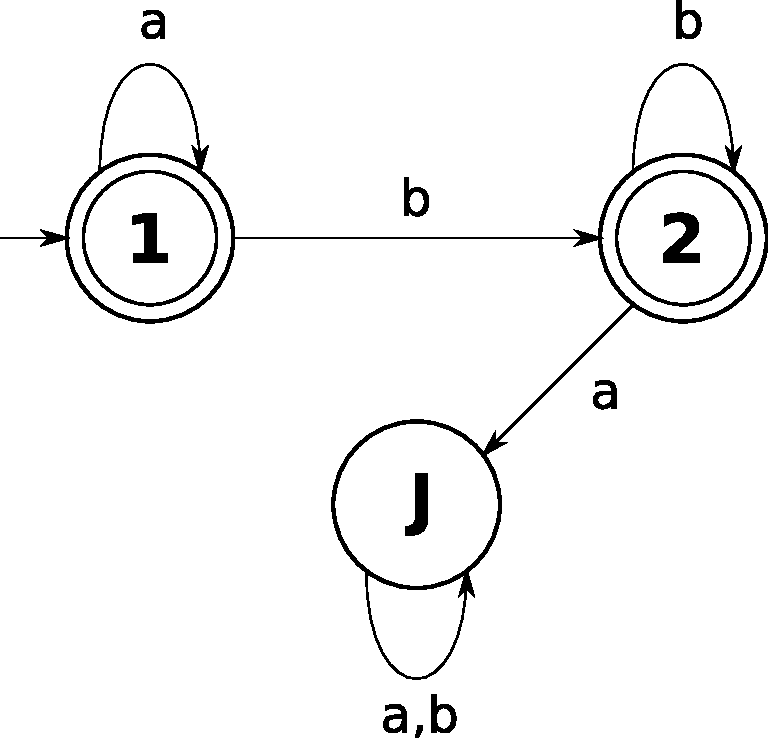
\includegraphics[width=0.8\linewidth]{Nerode.pdf}
	\end{minipage}
	\begin{minipage}{0.49\linewidth}
		Was sind die Nerode Äquivalenz\-klassen? \pause
		Wie komme ich in Zustand 1, 2, J? \pause
		$$\mathtt a^\ast, \mathtt a^\ast \mathtt b \mathtt b^\ast, \mathtt a^\ast \mathtt b \mathtt b^\ast \mathtt a \{\mathtt a, \mathtt b\}^\ast $$ \pause
		Wähle Vertreter! $$[\varepsilon], [\mathtt b], [\mathtt{ba}]$$
	\end{minipage}
\end{frame}

\begin{frame}{Noch ein Beispiel}
	Sei $L \subset A^\ast$ die Sprache 
	$$L = \{ \mathtt a^n \mathtt b \mathtt a^n \mid n \in \N\}$$ Wie sieht ein endlicher Automat dazu aus? \pause
	\begin{minipage}{0.49\linewidth}\vspace*{8em}
		\centering \vfill
		Argh! Es gibt keinen! \vspace*{4em}
	\end{minipage}\pause
	\begin{minipage}{0.49\linewidth}
		Was sind die Nerode Äquivalenz\-klassen? \pause
		Was passiert bei
		\begin{itemize}[<+->]
			\item $\mathtt a^i, i \in \N$
			\item $\mathtt a^i \mathtt b, i \in \N$
			\item dem Rest
		\end{itemize} \pause
		$$\{[\mathtt a^i] \mid i \in \N\} \cup \{[\mathtt a^i \mathtt b] \mid i \in \N\} \cup [\mathtt{ba}]$$
		
	\end{minipage}
\end{frame}




\section{Halbordnungen}
\subsection{Definition}
\begin{frame}
	\begin{Definition}
		Eine Relation $R\subseteq M\times M$ heißt \emph{antisymmetrisch}, wenn für alle $x,y\in M$ gilt $$ xRy \wedge yRx \implies x=y $$
	\end{Definition}
	\pause
	
	\begin{Definition}
		Eine Relation $R\subseteq M\times M$ heißt \emph{Halbordnung}, wenn sie 
		\begin{itemize}
			\item reflexiv
			\item antisymmetrisch
			\item transitiv 
		\end{itemize}
		ist. 
	\end{Definition}

\end{frame}

\subsection{Beispiel}
\begin{frame}
	\emph{Beispiel:} Sei $\sqsubseteq_p$ derart, dass für $v,w\in A^\ast$ gilt: $$ v \sqsubseteq_p w \iff \exists u\in A^\ast : vu = w $$ \pause
	\only<2-3>{Was sagt diese Halbordnung aus? \pause $v\sqsubseteq_p w$ heißt , dass $v$ ein Präfix von $w$ ist. \pause }
	\emph{Beweis}
	\only<4-6>{\begin{itemize}
		\only<4>{\item \emph{Reflexivität}
			$$ v \sqsubseteq_p v \iff \exists u\in A^\ast : vu = v \implies u = \varepsilon $$ Dies ist möglich, da $\varepsilon \in A^\ast$ }
		\only<5>{\item \emph{Antisymmetrie} \begin{align*}
			v\sqsubseteq_p w \wedge w\sqsubseteq_p v &\iff \exists u\in A^\ast : vu = w \wedge \exists \kappa\in A^\ast : w\kappa = v \\ &\implies w\kappa u = w \\ &\implies \kappa = u = \varepsilon \\ &\implies v = w 
		\end{align*}
		}
		\only<6>{ \item \emph{Transitivität}
		\begin{align*}
			v\sqsubseteq_p w \wedge w\sqsubseteq_p x &\iff \exists u\in A^\ast : vu = w \wedge \exists \kappa\in A^\ast : w\kappa = x \\ &\implies vu\kappa = x \\ &\overset{\alpha=u\kappa}{\iff} \exists \alpha\in A^\ast: v\alpha = x \\ &\iff v\sqsubseteq_p x
		\end{align*}
		 }
	\end{itemize}}
\end{frame}

\subsection{Aufgaben}
\begin{frame}
	Zeigen Sie, dass $\leq $ und $\subseteq$ Halbordnungen sind.
\end{frame}
\subsection{Lösung}
\begin{frame}
	Betrachte die Relation $\leq$. Dann gilt mit $$ a\leq b \iff \exists \alpha \in \R^+_0 : a + \alpha = b $$  \pause
	\only<2-4>{
	\begin{itemize}
		\only<2>{\item \emph{Reflexivität}
		\begin{align*}
			a\leq a & \iff \exists \alpha\geq 0 : a + \alpha = a \\ &\implies \alpha = 0 \in \R^+_0
		\end{align*}
		}
		\only<3>{\item
		\emph{Antisymmetrie}
		\begin{align*}
			a \leq b \wedge b \leq a &\iff \exists \alpha, \beta \in\R^+_0 : a + \alpha = b \wedge b + \beta = a \\ &\implies a + \alpha + \beta = a \\ &\overset{\alpha,\beta\geq 0}{\implies} \alpha = \beta = 0 \\ &\implies a = b
		\end{align*}
		}
		\only<4>{\item
		\emph{Transitivität}
		\begin{align*}
			a \leq b \wedge b \leq c &\iff \exists \alpha,\beta \in\R^+_0 : a + \alpha = b \wedge b+\beta = c \\ &\implies a + \alpha + \beta = c \\ &\overset{\gamma=\alpha+\beta}{\implies} \exists \gamma \in\R^+_0 : a + \gamma = c \\ &\implies a\leq c
		\end{align*}
		}
	\end{itemize}	
	}
\end{frame}

\begin{frame}
	Betrachte die Relation $\subseteq$. Dann gilt \pause
	\only<2-9>{
	\begin{itemize}
		\only<2-3>{\item \emph{Reflexivität}
		\begin{align*}
			\only<2>{A \subseteq A &\iff \left( A\subset A \right) \vee \left( A = A \right)}
			\only<3>{A \subseteq A &\iff \left(\textcolor{red}{A\subset A}\right) \vee \left(\textcolor{green}{A = A}\right)}
		\end{align*}
		\only<3>{Dies ist eine wahre Aussage.}
		}
		\only<4-8>{\item
		\emph{Antisymmetrie}
		\begin{align*}
			\only<4-8>{
			A\subseteq B \wedge B\subseteq A \Leftrightarrow & \left( A \subset B \vee A = B \right) \wedge \left( B\subset A \vee B = A \right)
		}
		 \only<5-8>{\\ \Leftrightarrow &  \left( (A\subset B) \wedge \left( B\subset A \vee B = A \right)\right) \\
		 &\vee \left((A = B) \wedge \left( B\subset A \vee B = A \right) \right) \\} 
		\only<6>{\Leftrightarrow &   \left((A\subset B)\wedge (B\subset A) \right) \vee \left( (A\subset B) \wedge (B=A) \right)   \\
		 & \vee  \left( (A=B)\wedge (B\subset A) \right) \vee \left( (A=B) \wedge (B=A) \right)  } 
		\only<7-8>{\Leftrightarrow &   \textcolor{red}{\left((A\subset B)\wedge (B\subset A) \right)} \vee \textcolor{red}{\left( (A\subset B) \wedge (B=A) \right)}   \\
		 & \vee  \textcolor{red}{\left( (A=B)\wedge (B\subset A) \right)} \vee \textcolor{green}{\left( (A=B) \wedge (B=A) \right)}
		 }
		\end{align*}
		}
		\only<8>{Also folgt $$ A\subseteq B \wedge B\subseteq A \implies A = B $$ Dies benutzen wir um Mengengleichheit zu zeigen.
		}
		\only<9>{
		\item
		\emph{Transitivität} 
		\begin{align*}
			A\subseteq B \wedge B\subseteq C &\iff \forall a\in A : a\in B \wedge \forall b\in B : b\in C \\ &\implies a \in C \\ &\implies A\subseteq C
		\end{align*}
		}
	\end{itemize}	
	}
\end{frame}

\subsection{Potenzmengen}
\begin{frame}
	\begin{Definition}
		Als \emph{Potenzmenge} $\mathcal{P}(X)$ ist die Menge aller Teilmengen von $X$ ist definiert. $$ \mathcal{P}(X) = \{ U | U\subseteq X\} $$
		Weitere Notation : $ \mathcal{P}(X) = 2^X $ \\
		
		Für die Mächtigkeit finden wir $$ \vert \mathcal{P}(X) \vert = 2^{\vert X \vert} $$
	\end{Definition} 
	\pause 
	\emph{Beispiel}
	$$ \mathcal{P}(\{a,b\}) = \{ \emptyset, \{a\}, \{b\}, \{a,b\} \} $$
	\pause
	$$\mathcal{P}(\{a,b,c\}) = \{ \emptyset, \{a\}, \{b\}, \{c\}, \{a,b\}, \{a,c\}, \{b,c\}, \{a,b,c\} \} $$
\end{frame}

\begin{frame}
	Betrachten wir nun die Halbordnung $\subseteq$ auf der Menge $\mathcal{P}(\{a,b,c\})$ \pause
	\begin{figure}[H]
		\centering
		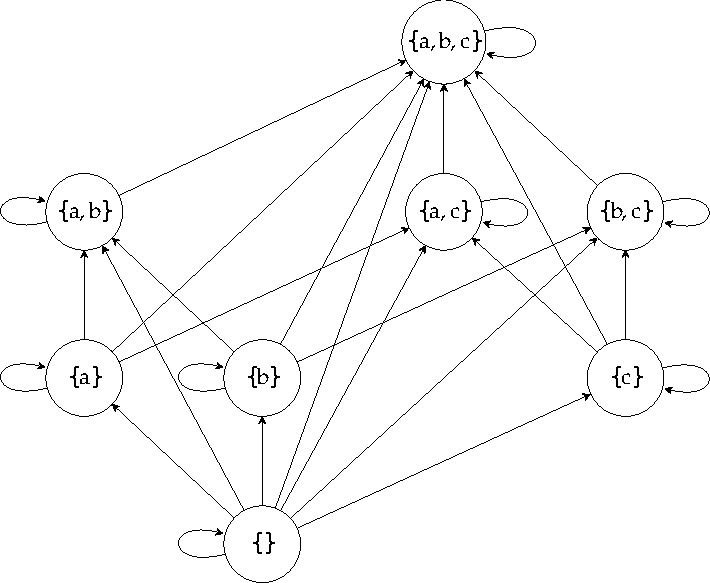
\includegraphics[scale=0.7]{../figures/halbordnungen/Halbordnung.pdf}
	\end{figure} \pause
	Wird doch recht bald unübersichtlich!
\end{frame}

\section{Hasse-Diagramm}
\begin{frame}
Lassen wir nun einfach die Kanten weg, die sich durch Transitivität und Reflexivität ergeben \pause
\begin{figure}[H]
	\centering
	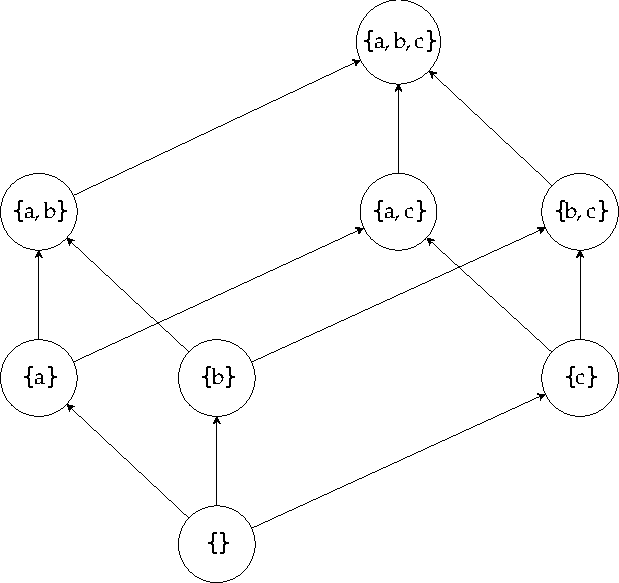
\includegraphics[scale=0.65]{../figures/halbordnungen/Hasse1.pdf}
\end{figure} \pause
Dies nennen wir das \emph{Hasse-Diagramm}.
\end{frame}

\subsection{Definition}
\begin{frame}
	\begin{Definition}
		Eine Diagramm einer Halbordnung $\sqsubseteq$ auf einer Menge $M$ heißt \emph{Hasse-Diagramm}, wenn es im Diagramm eine Kante gibt von $a$ nach $b$, $a,b\in M$, sofern gilt $$ \nexists c\in M : a\sqsubseteq c \sqsubseteq b $$
	\end{Definition} \pause
	
	\begin{Definition}
		Es sei $(M,\sqsubseteq)$ eine halbgeordnete Menge und $T\subseteq M$. Ein Element $x\in T$ heißt 
		\begin{itemize}
			\item \emph{minimales Element} von $T$, wenn es kein $y\in T, y\neq x$ gibt, mit $y\sqsubseteq x$.
			\item \emph{maximales Element} von $T$, wenn es kein $y\in T, y\neq x$ gibt, mit $x\sqsubseteq y$.
			\item \emph{größtes Element} von $T$, wenn für alle $y\in T$ gilt $y\sqsubseteq x$
			\item \emph{kleinstes Element} von $T$, wenn für alle $y\in T$ gilt $x\sqsubseteq y$
		\end{itemize}
	
	\end{Definition}
\end{frame}

%\begin{frame}
%	Beispiele an der Tafel zu $\sqsubseteq = \subseteq$ und $ M \in \{ \mathcal{P}(\{a\}), \mathcal{P}(\{a\})\cup \{d\}, \{a\}\cup\{d\} \}$
%\end{frame}



\subsection{Aufgabe}
\begin{frame}{WS 10/11}
	Geben Sie das Hasse-Diagramm einer Halbordnung auf einer dreielementigen Menge an, die genau zwei maximale und zwei minimale Elemente besitzt.
\end{frame}
\subsection{Lösung}
\begin{frame}
	\begin{figure}[H]
		\centering
		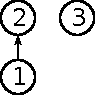
\includegraphics[scale=0.7]{../figures/halbordnungen/Loesung.pdf}
	\end{figure}
\end{frame}

%% Was ihr nun wissen solltet
\section{Schluss}
\begin{frame}
	\frametitle{Was ihr nun wissen solltet}
	\begin{itemize}
		\item Was ein Hasse-Diagramm ist
		\item Das man manchmal Triviales wirklich beweisen muss
		\item Das es nun zu Ende ist.
	\end{itemize}
\end{frame}

%% Letzte Seite
\lastframe{0.45}{xkcd/turing_test.png}{http://xkcd.com/329/}

\end{document}